%!TEX root = ../dissertation.tex


\chapter{Magneto-thermal transport}
\label{ch:magneto-thermal_transport}

goal is to develop thermal probes for magnetic systems in 2D because thermal transport is sensitive to things electric transport isnt (entropy, hydrodynamics, non-fermi liquid behavior, Fermi surface changes). Johnson noise and joule heating are very sensitive to local quantum effects as they can probe a weighted average of the entire sample.


in degenerate semi conductors and metals WF should hold under Fermi liquid in magnetic field even down to quantum of conductance. cite

discuss WF in graphene magnetic field, cite.

\section{Classical Hall Effect}
magnetic fields change the current profile. heating profile. 
Average temperature is effected but Johnson noise temperature is not
in a linear, classical system; factor of 12 holds
plots of temperature and potential profiles

\begin{figure}
\centering
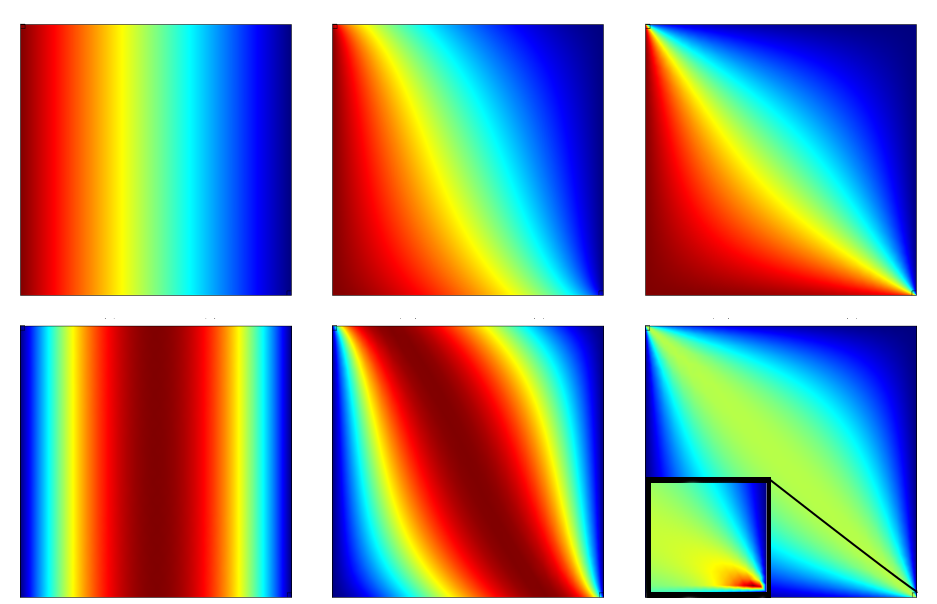
\includegraphics[width=100mm]{figures/magneto/Hall_T_V.png}
\caption{caption}
\label{fig:m_Hall_profiles}
\end{figure}

\section{Sample characteristics}

\begin{figure}
\centering
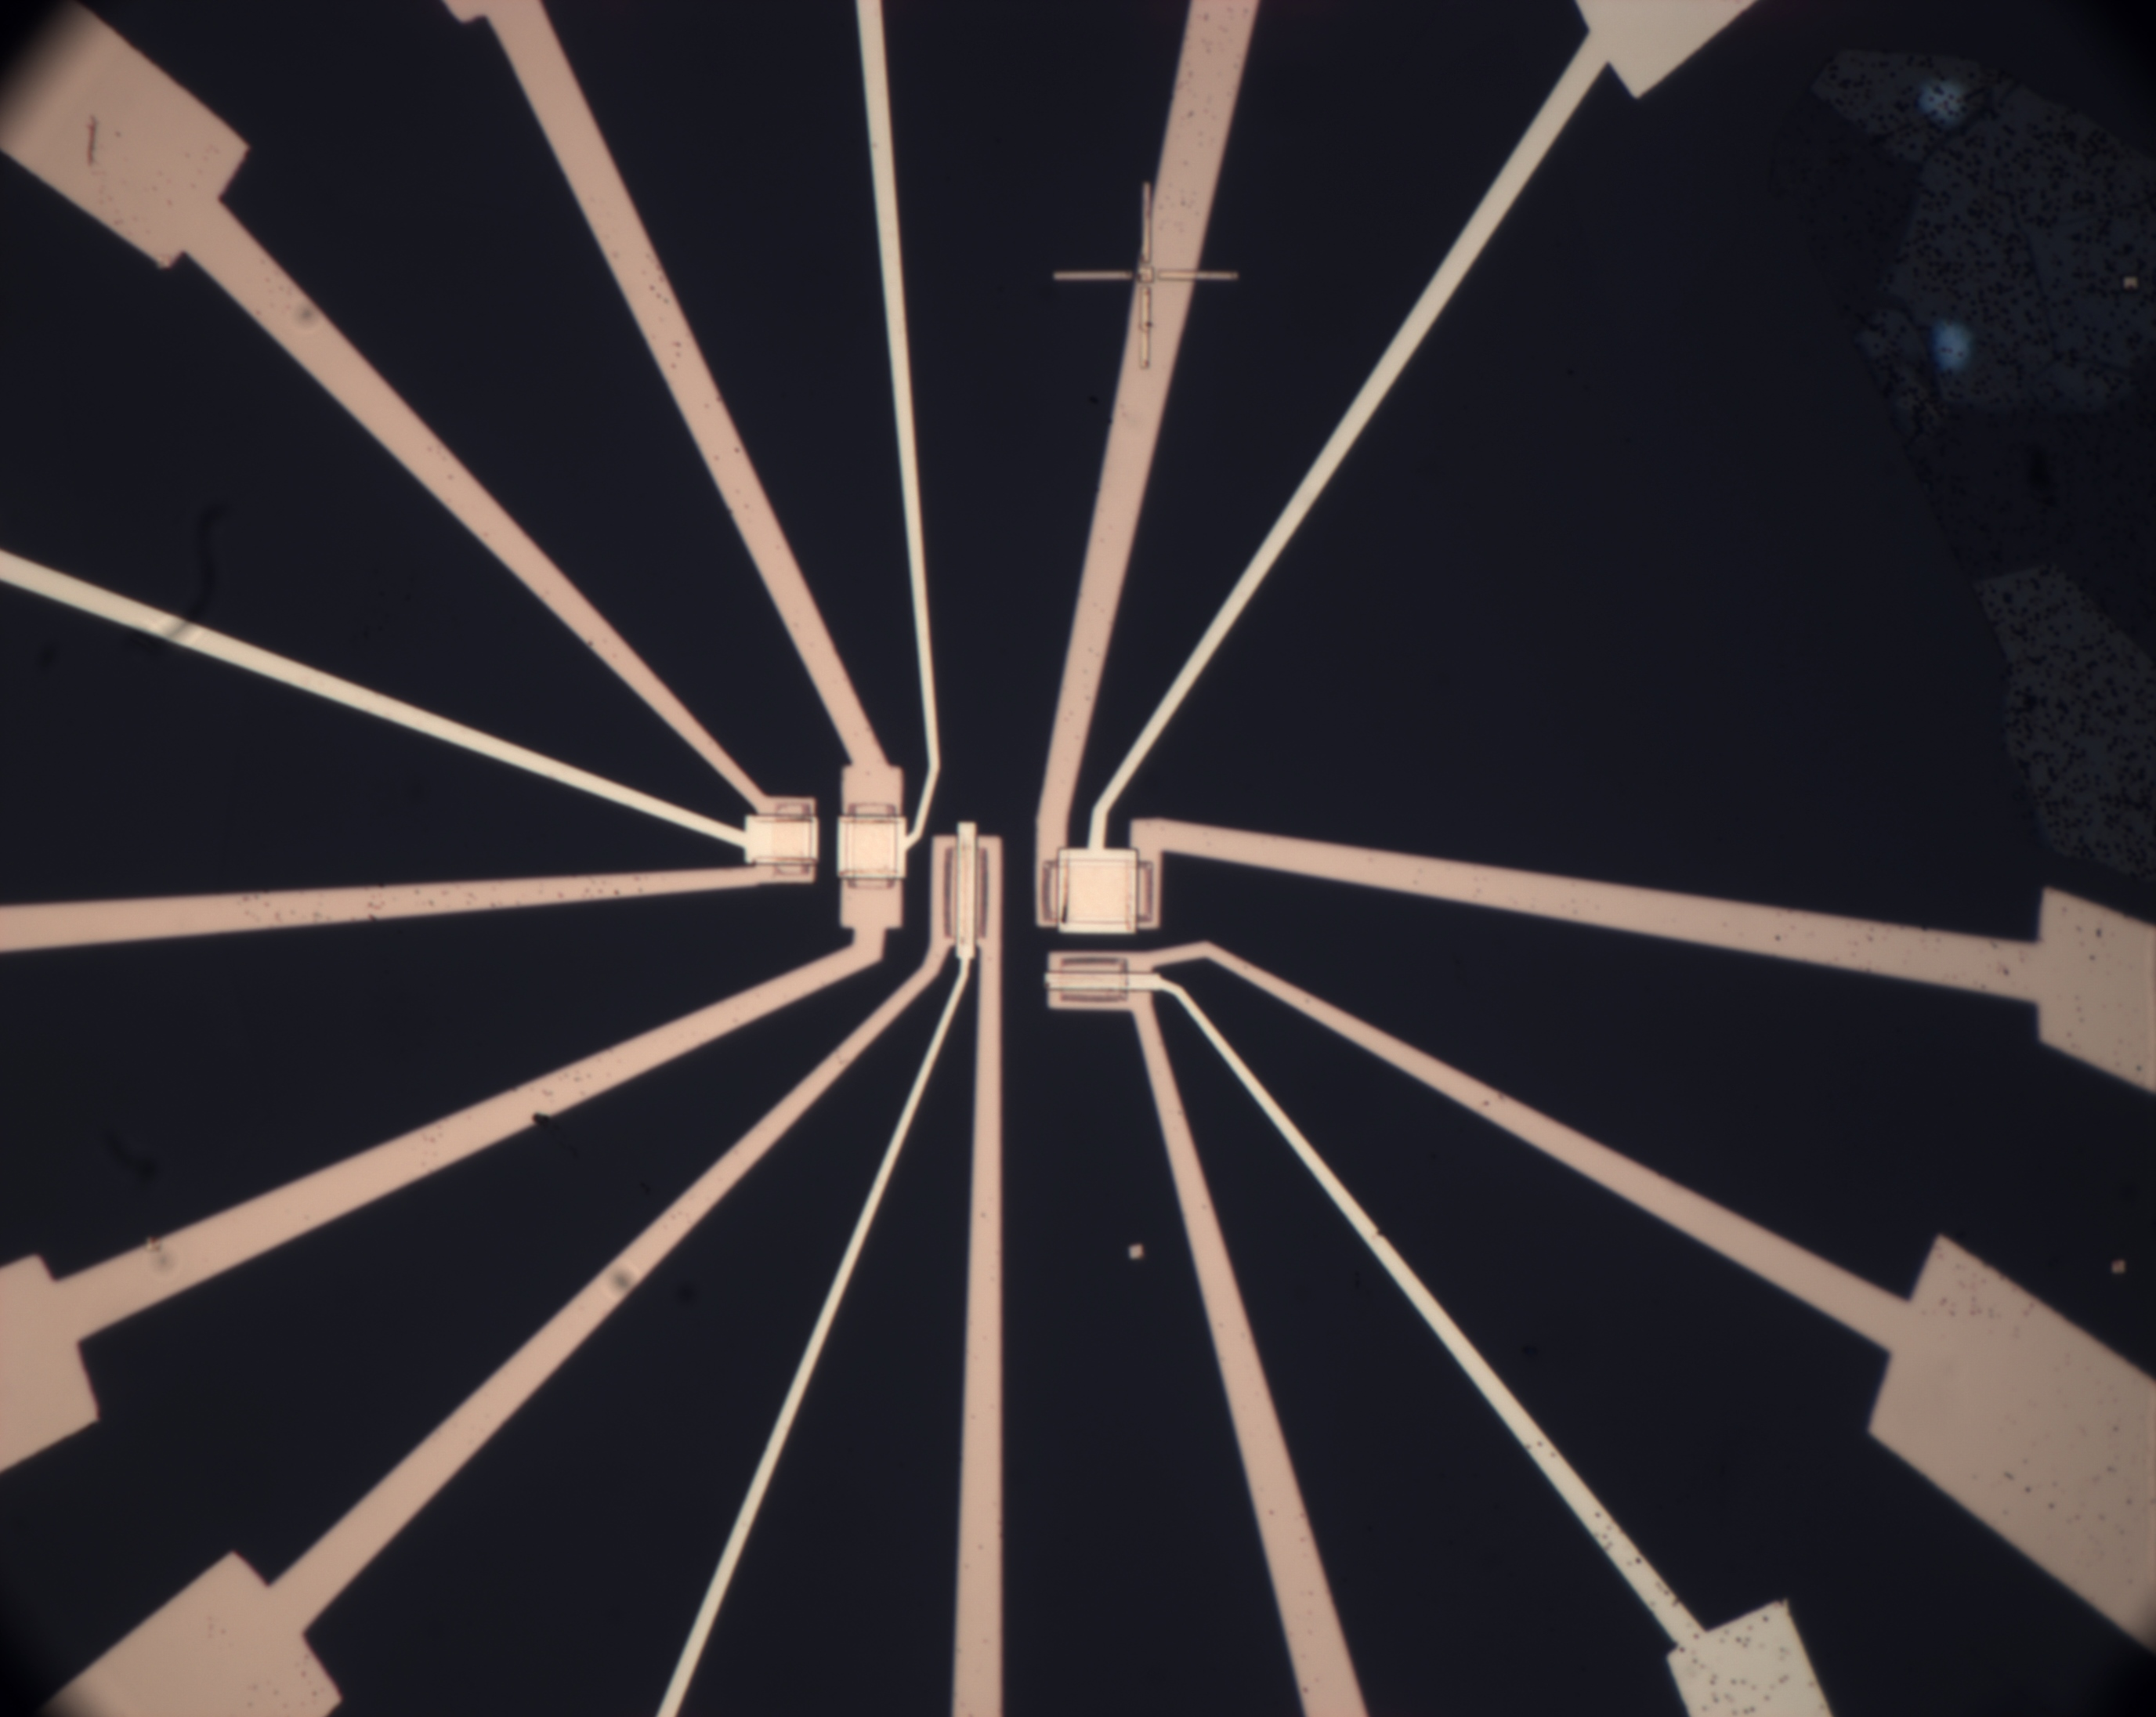
\includegraphics[width=100mm]{figures/magneto/100x.jpg}
\caption{caption}
\label{fig:m_Giorgio}
\end{figure}

\begin{figure}
\centering
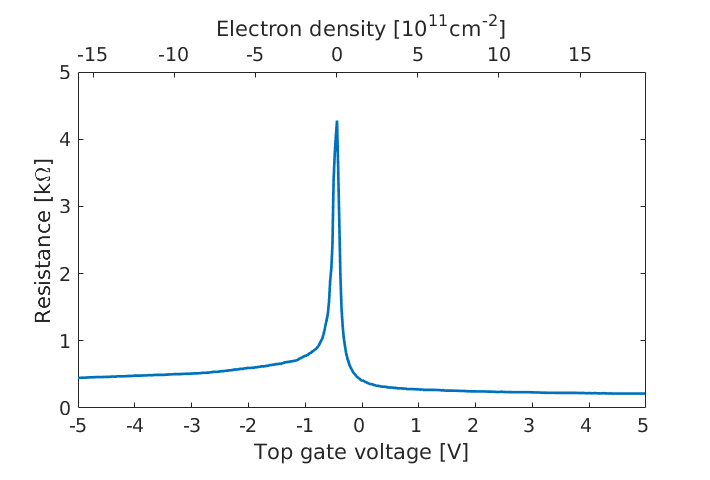
\includegraphics[width=100mm]{figures/magneto/R.png}
\caption{caption}
\label{fig:m_R}
\end{figure}

\begin{figure}
\centering
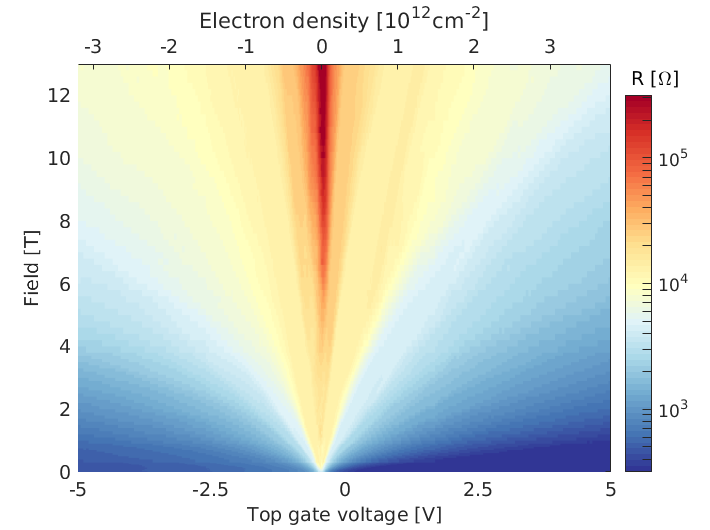
\includegraphics[width=100mm]{figures/magneto/Fan_R.png}
\caption{caption}
\label{fig:m_Fan_R}
\end{figure}

\begin{figure}
\centering
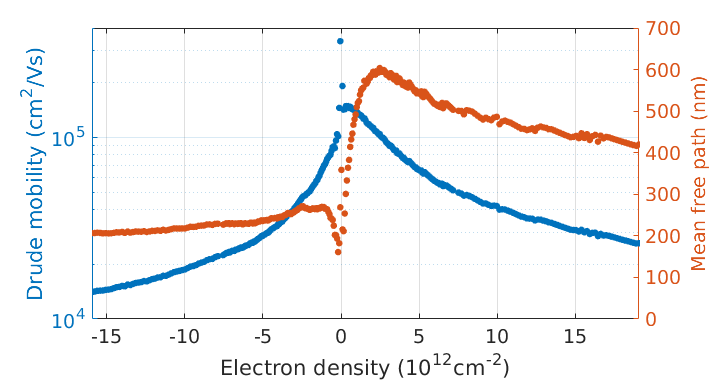
\includegraphics[width=100mm]{figures/magneto/mobility_mfp_1K.png}
\caption{caption}
\label{fig:m_mobility}
\end{figure}

\section{Electrical noise in high fields}

\begin{figure}
\centering
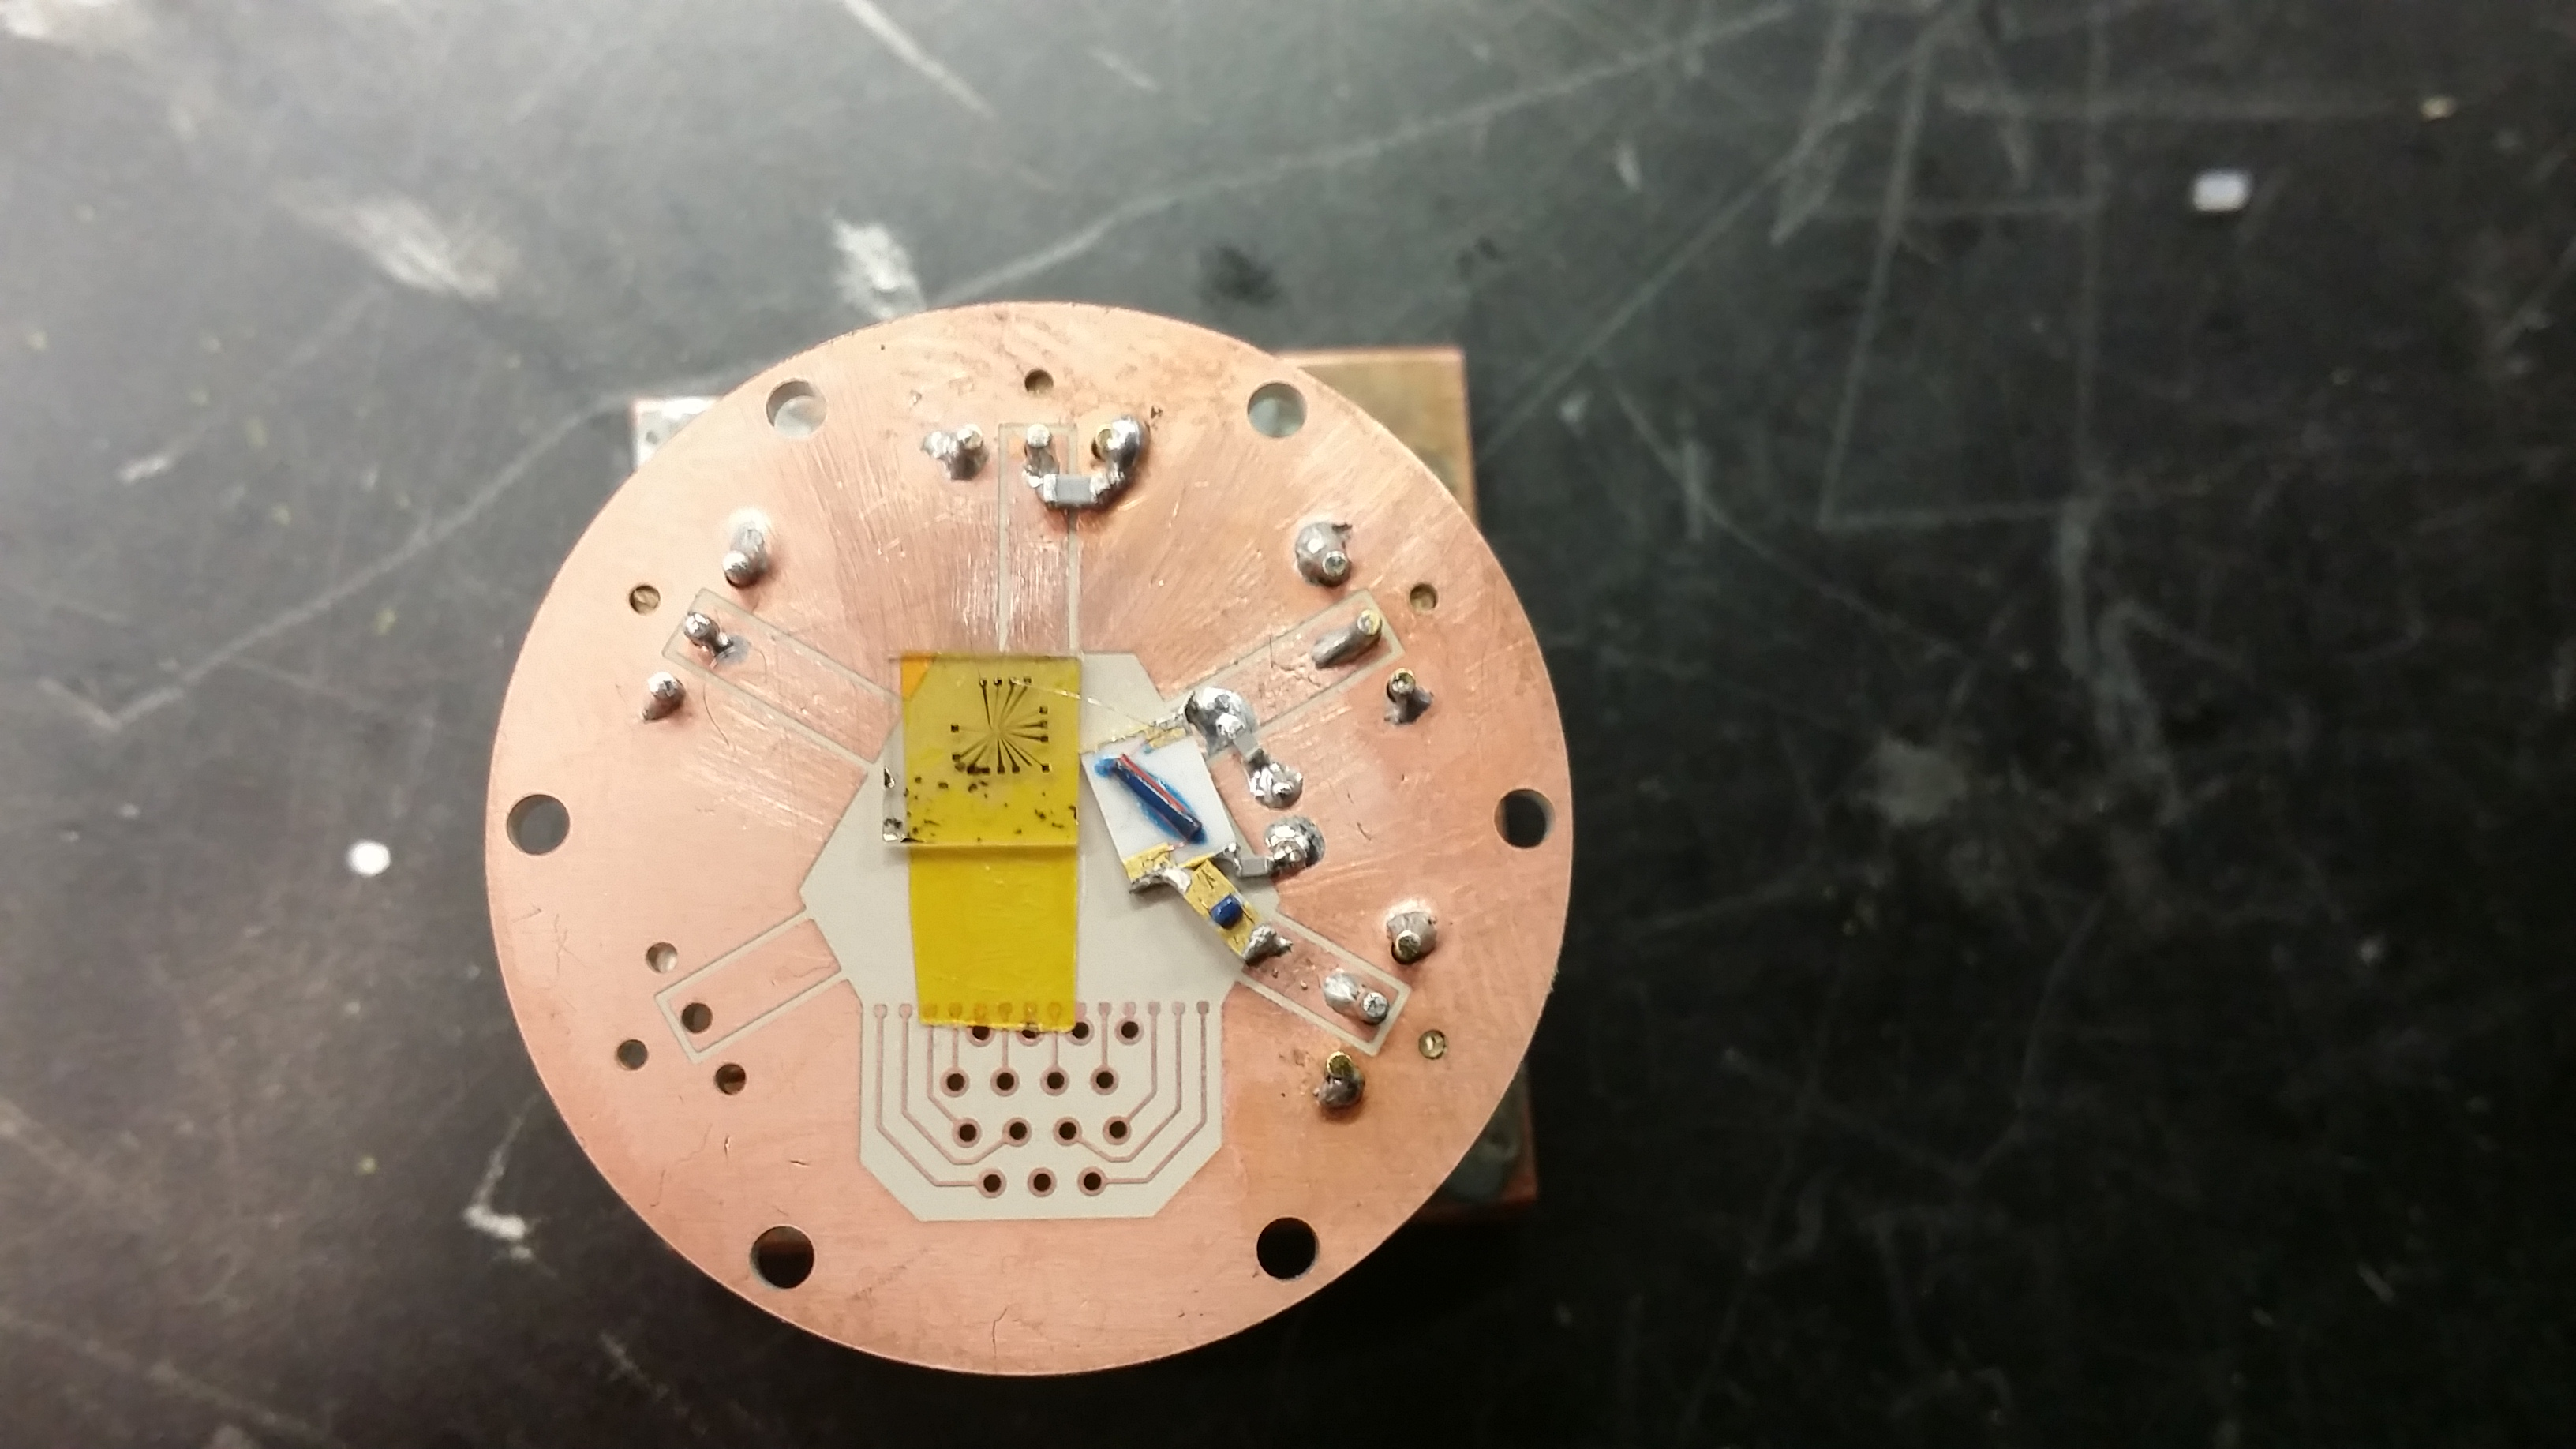
\includegraphics[width=100mm]{figures/magneto/picture_matching_ceramic.jpg}
\caption{caption}
\label{fig:m_matching}
\end{figure}

\begin{figure}
\centering
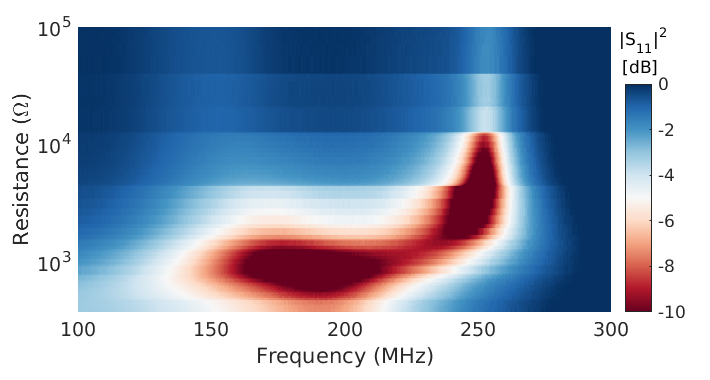
\includegraphics[width=100mm]{figures/magneto/S11_plot.png}
\caption{caption}
\label{fig:m_S11}
\end{figure}

\begin{figure}
\centering
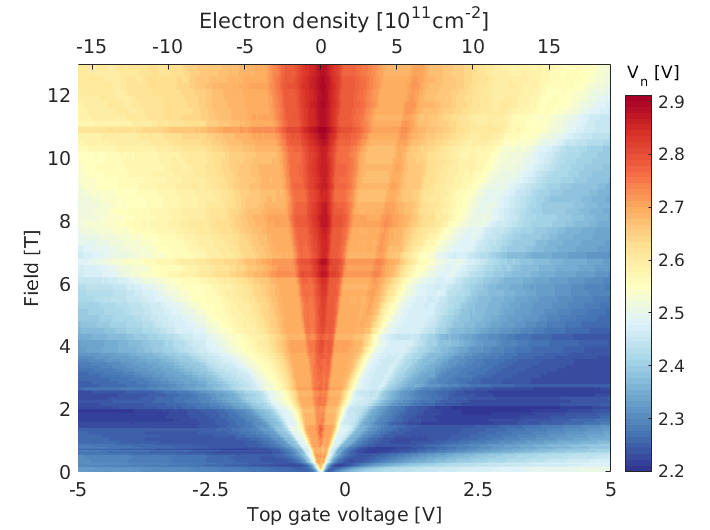
\includegraphics[width=100mm]{figures/magneto/Fan_VNdc.png}
\caption{caption}
\label{fig:m_VNdc}
\end{figure}

\section{Magneto-thermal conductance}

\begin{figure}
\centering
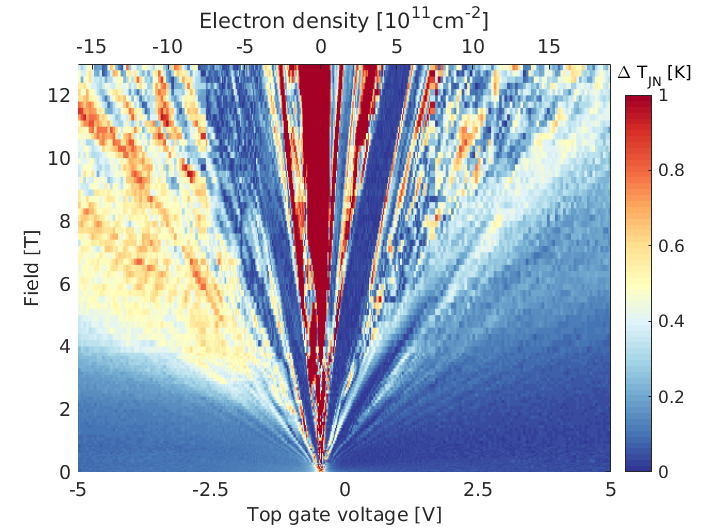
\includegraphics[width=100mm]{figures/magneto/Fan_DT.png}
\caption{caption}
\label{fig:m_DT}
\end{figure}

\begin{figure}
\centering
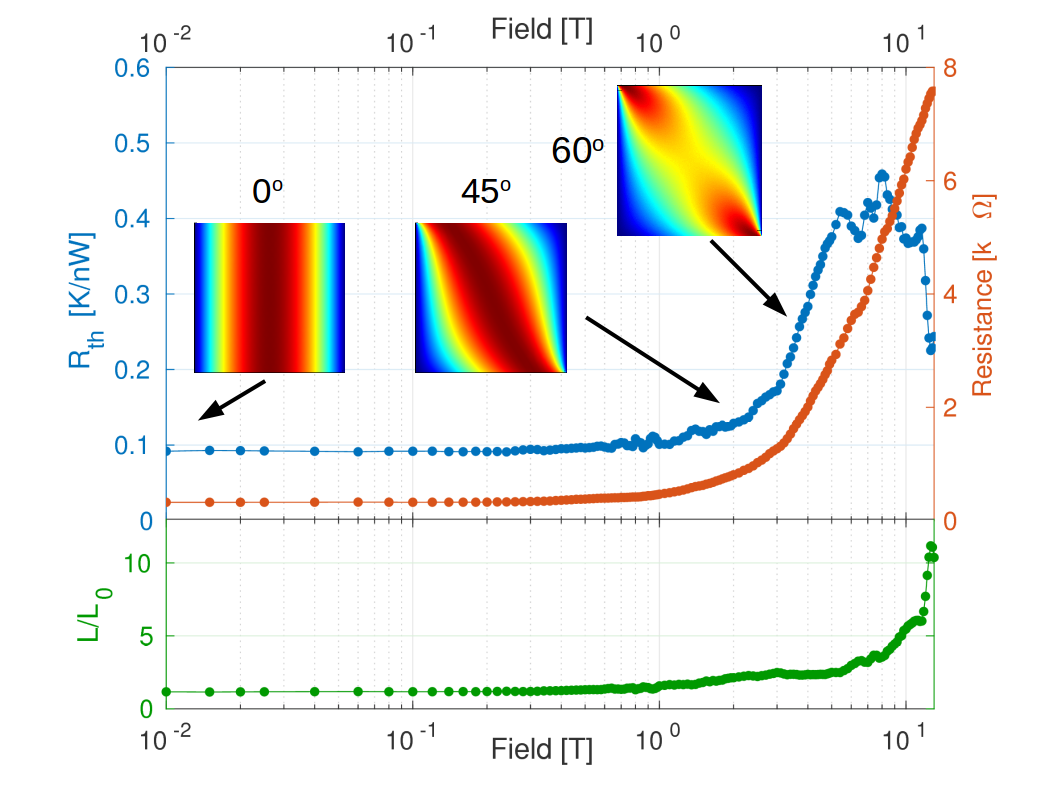
\includegraphics[width=100mm]{figures/magneto/High_density.png}
\caption{caption}
\label{fig:m_high_density}
\end{figure}

\begin{figure}
\centering
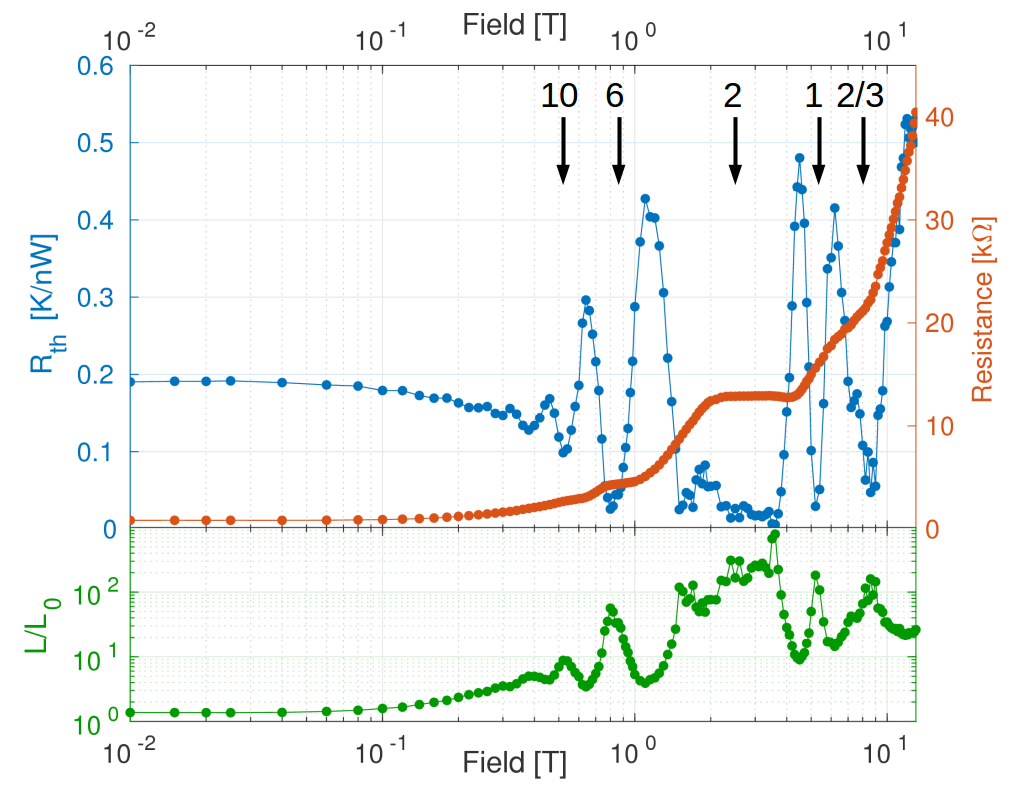
\includegraphics[width=100mm]{figures/magneto/Low_density.png}
\label{fig:m_low_density}
\end{figure}

\begin{figure}
\centering
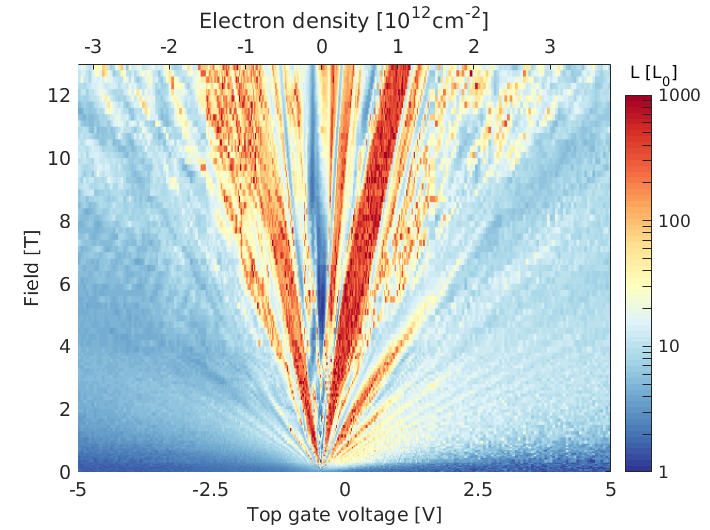
\includegraphics[width=100mm]{figures/magneto/Fan_L.png}
\caption{caption}
\label{fig:m_L}
\end{figure}

\begin{figure}
\centering
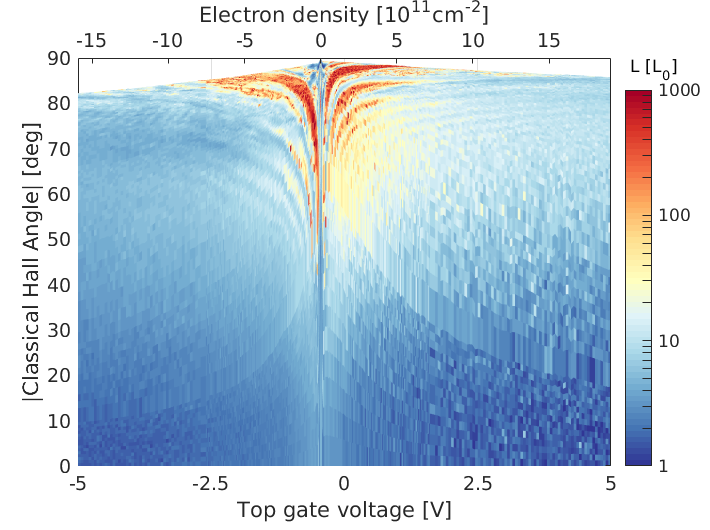
\includegraphics[width=100mm]{figures/magneto/L_n_Ha.png}
\caption{caption}
\label{fig:m_L_n_Ha}
\end{figure}





\newthought{There's something to be said} for having a good opening line. 
